% Options for packages loaded elsewhere
\PassOptionsToPackage{unicode}{hyperref}
\PassOptionsToPackage{hyphens}{url}
\PassOptionsToPackage{dvipsnames,svgnames*,x11names*}{xcolor}
%
\documentclass[
  russian,
  a4paper,
  russian]{scrreprt}
\usepackage{lmodern}
\usepackage{setspace}
\setstretch{1.2}
\usepackage{amssymb,amsmath}
\usepackage{ifxetex,ifluatex}
\ifnum 0\ifxetex 1\fi\ifluatex 1\fi=0 % if pdftex
  \typeout{Setting Fonts for pdftex}
  \usepackage[T2A,T1]{fontenc}
  \usepackage[utf8]{inputenc}
  \usepackage{textcomp} % provide euro and other symbols
\else % if luatex or xetex
  \typeout{Setting Fonts for luatex or xetex}
  \usepackage{unicode-math}
  \defaultfontfeatures{Scale=MatchLowercase}
%   \defaultfontfeatures[\rmfamily]{Ligatures=TeX,Scale=1}
  \setmainfont[Script=Cyrillic]{Times New Roman}
  \setmonofont[
    Contextuals={Alternate} % Activate the calt feature
  ]{Fira Code}
  \makeatletter
  \renewcommand*\verbatim@nolig@list{} % Empty the no-ligature list
  \makeatother
\fi
% Use upquote if available, for straight quotes in verbatim environments
\IfFileExists{upquote.sty}{\usepackage{upquote}}{}
\IfFileExists{microtype.sty}{% use microtype if available
  \usepackage[]{microtype}
  \UseMicrotypeSet[protrusion]{basicmath} % disable protrusion for tt fonts
}{}

\makeatletter
\@ifundefined{KOMAClassName}{% if non-KOMA class
  \IfFileExists{parskip.sty}{%
    \usepackage{parskip}
  }{% else
    \setlength{\parindent}{0pt}
    \setlength{\parskip}{6pt plus 2pt minus 1pt}}
}{% if KOMA class
  \KOMAoptions{parskip=half}}
\makeatother

\usepackage{xcolor}
\IfFileExists{xurl.sty}{\usepackage{xurl}}{} % add URL line breaks if available
\IfFileExists{bookmark.sty}{\usepackage{bookmark}}{\usepackage{hyperref}}
\hypersetup{
  pdftitle={Домашняя работа по Математической Статистике},
  pdfauthor={Митин Арсений (3 курс, СКБ171)},
  pdflang={ru},
  pdfkeywords={Statistics},
  colorlinks=true,
  linkcolor=blue,
  filecolor=Maroon,
  citecolor=Blue,
  urlcolor=Blue,
  pdfcreator={LaTeX via pandoc}}
\urlstyle{same} % disable monospaced font for URLs
\usepackage[margin=2.5cm,includehead=true,includefoot=true]{geometry}
\usepackage{textcomp}
\usepackage{listings}
% \usepackage[space=true]{accsupp} % http://ctan.org/pkg/accsupp
% \providecommand{\nocopynumber}[1]{
%   \BeginAccSupp{method=escape,ActualText={}}
%   #1
%   \EndAccSupp{}
% }
\newcommand{\passthrough}[1]{#1}
\lstset{defaultdialect=[5.3]Lua}
\lstset{defaultdialect=[x86masm]Assembler}

% https://github.com/tonsky/FiraCode/wiki/LaTeX-instructions
\usepackage{lstfiracode} % for FiraCodeStyle
\usepackage{MnSymbol} % for \rhookswarrow
\lstset{
  language=Haskell,
  backgroundcolor   = \color[HTML]{FFFFFF},
  basicstyle        = \ttfamily\scriptsize\color[HTML]{000000},
  breaklines        = true,
  breakatwhitespace = true,
  breakautoindent   = true,
  commentstyle      = \color[HTML]{009900},
  frame             = l,
  framesep          = 7pt,
  keepspaces        = true,
  keywordstyle      = \color[HTML]{000099},
  numbers           = left,
  numberstyle       = \small\color[HTML]{808080},%\nocopynumber,
  numbersep         = 10pt,
  prebreak          = \raisebox{0ex}[0ex][0ex]{\ensuremath{\rhookswarrow}},
  postbreak         = \raisebox{0ex}[0ex][0ex]{\ensuremath{\hookrightarrow\space}},
  rulecolor         = \color[HTML]{808080},
  showspaces        = false,
  showstringspaces  = false,
  stringstyle       = \color[HTML]{009966},
  style             = FiraCodeStyle,
  tabsize           = 2,
  upquote           = true,
}

\usepackage[
  symbol=$\uparrow$,
  numberlinked=false,
]{footnotebackref}

\usepackage{graphicx,grffile}
\makeatletter
\def\maxwidth{\ifdim\Gin@nat@width>\linewidth\linewidth\else\Gin@nat@width\fi}
\def\maxheight{\ifdim\Gin@nat@height>\textheight\textheight\else\Gin@nat@height\fi}
\makeatother
% Scale images if necessary, so that they will not overflow the page
% margins by default, and it is still possible to overwrite the defaults
% using explicit options in \includegraphics[width, height, ...]{}
\setkeys{Gin}{width=\maxwidth,height=\maxheight,keepaspectratio}
% Set default figure placement to htbp
\makeatletter
\def\fps@figure{htbp}
\makeatother
\setlength{\emergencystretch}{3em} % prevent overfull lines
\providecommand{\tightlist}{%
  \setlength{\itemsep}{0pt}\setlength{\parskip}{0pt}}
\setcounter{secnumdepth}{2}



% Make use of float-package and set default placement for figures to H.
% The option H means 'PUT IT HERE' (as  opposed to the standard h option which means 'You may put it here if you like').
\usepackage{float}
\floatplacement{figure}{H}

\newfontfamily\cyrillicfont{Times New Roman}
\RedeclareSectionCommand[
  beforeskip=-10pt plus -2pt minus -1pt,
  afterskip=1sp plus -1sp minus 1sp,
  font=\normalfont\itshape]{paragraph}
\RedeclareSectionCommand[
  beforeskip=-10pt plus -2pt minus -1pt,
  afterskip=1sp plus -1sp minus 1sp,
  font=\normalfont\scshape,
  indent=0pt]{subparagraph}
\makeatletter
\@ifpackageloaded{subfig}{}{\usepackage{subfig}}
\@ifpackageloaded{caption}{}{\usepackage{caption}}
\captionsetup[subfloat]{margin=0.5em}
\AtBeginDocument{%
\renewcommand*\figurename{Figure}
\renewcommand*\tablename{Table}
}
\AtBeginDocument{%
\renewcommand*\listfigurename{List of Figures}
\renewcommand*\listtablename{List of Tables}
}
\newcommand*\listoflistings\lstlistoflistings
\AtBeginDocument{%
\renewcommand*{\lstlistlistingname}{List of Listings}
}
\makeatother
\ifnum 0\ifxetex 1\fi\ifluatex 1\fi=0 % if pdftex
  \typeout{Setting Languages for pdftex}
  \usepackage[shorthands=off,main=russian]{babel}
\else % if luatex or xetex
  \typeout{Setting Languages for luatex or xetex}
  \usepackage{polyglossia}
  
  % See issue https://github.com/reutenauer/polyglossia/issues/127
  \renewcommand*\familydefault{\sfdefault}

  \setmainlanguage[]{russian}
%
% When using babel or polyglossia with biblatex, loading csquotes is recommended
% to ensure that quoted texts are typeset according to the rules of your main language.
%
\usepackage{csquotes}
\fi

\title{Домашняя работа по Математической Статистике}
\author{Митин Арсений (3 курс, СКБ171)}
\date{26.10.2019}


\usepackage{fancyhdr}
\pagestyle{fancy}
\fancyhf{}
\fancyhead[LO,LE]{\leftmark}
\fancyhead[RO,RE]{\rightmark}
\fancyfoot[C]{\thepage}
\renewcommand{\headrulewidth}{0.4pt}
\renewcommand{\footrulewidth}{0.4pt}


\begin{document}
\maketitle

\newpage
{
\hypersetup{linkcolor=}
\setcounter{tocdepth}{2}
\tableofcontents
\newpage
}
\providecommand{\mathFunc}[4]{#1\left#2\, #3 \,\right#4}
\providecommand{\mathbbFunc}[4]{\mathFunc{\mathbb{#1}}{#2}{#3}{#4}}
\providecommand{\mathrmFunc}[4]{\mathFunc{\mathrm{#1}}{#2}{#3}{#4}}
\providecommand{\Prob}[1]{\mathbbFunc{P}{(}{#1}{)}}
\providecommand{\Expect}[1]{\mathbbFunc{E}{[}{#1}{]}}
\providecommand{\Var}[1]{\mathrmFunc{Var}{[}{#1}{]}}

\hypertarget{ux437ux430ux434ux430ux43dux438ux435-1}{%
\chapter{Задание №1}\label{ux437ux430ux434ux430ux43dux438ux435-1}}

\hypertarget{ux432ux44bux431ux43eux440-ux440ux430ux441ux43fux440ux435ux434ux435ux43bux435ux43dux438ux439}{%
\section{Выбор
распределений}\label{ux432ux44bux431ux43eux440-ux440ux430ux441ux43fux440ux435ux434ux435ux43bux435ux43dux438ux439}}

Выбранные распределения:

\begin{itemize}
\tightlist
\item
  Дискретное: \emph{гипергеометрическое}
\item
  Непрерывное: \emph{нормальное}
\end{itemize}

\hypertarget{ux43eux43fux438ux441ux430ux43dux438ux435-ux43eux441ux43dux43eux432ux43dux44bux445-ux445ux430ux440ux430ux43aux442ux435ux440ux438ux441ux442ux438ux43a-ux440ux430ux441ux43fux440ux435ux434ux435ux43bux435ux43dux438ux439}{%
\section{Описание основных характеристик
распределений}\label{ux43eux43fux438ux441ux430ux43dux438ux435-ux43eux441ux43dux43eux432ux43dux44bux445-ux445ux430ux440ux430ux43aux442ux435ux440ux438ux441ux442ux438ux43a-ux440ux430ux441ux43fux440ux435ux434ux435ux43bux435ux43dux438ux439}}

\hypertarget{ux433ux438ux43fux435ux440ux433ux435ux43eux43cux435ux442ux440ux438ux447ux435ux441ux43aux43eux435-ux440ux430ux441ux43fux440ux435ux434ux435ux43bux435ux43dux438ux435}{%
\subsection{Гипергеометрическое
распределение}\label{ux433ux438ux43fux435ux440ux433ux435ux43eux43cux435ux442ux440ux438ux447ux435ux441ux43aux43eux435-ux440ux430ux441ux43fux440ux435ux434ux435ux43bux435ux43dux438ux435}}

Гипергеометрическое распределение - дискретное распределение,
описывающее вероятность события, при котором ровно \(k\) из \(n\)
случайно выбранных элементов окажутся \emph{помеченными}, при этом
выборка осуществляется из множества мощности \(N\), в котором
присутствует \(m\) помеченных элементов. Считается, что каждый из
элементов может быть выбран с одинаковой вероятностью \(\frac{1}{N}\).
Запишем это формально: \[\begin{gathered}
    N \in \mathbb{N},\ m \in \overline{0, N},\ n \in \overline{0, N},\\
    k \in \overline{0, n}
\end{gathered}\] Тогда \(HG(D, N, n)\) описывает вероятность события,
при котором ровно \(k\) из \(n\) элементов выборки окажутся
\emph{помеченными}: \[\begin{gathered}
    \left\{\xi \sim HG(N, m, n) \right\}\\
    \Updownarrow\\
    \left\{\mathbb{P}\left(\, \xi=k \,\right) = \frac{\binom{m}{k}\binom{N-m}{n-k}}{\binom{N}{n}}\right\}
\end{gathered}\]

\hypertarget{ux43cux430ux442ux435ux43cux430ux442ux438ux447ux435ux441ux43aux43eux435-ux43eux436ux438ux434ux430ux43dux438ux435-ux433ux438ux43fux435ux440ux433ux435ux43eux43cux435ux442ux440ux438ux447ux435ux441ux43aux43eux433ux43e-ux440ux430ux441ux43fux440ux435ux434ux435ux43bux435ux43dux438ux44f}{%
\subsubsection{Математическое ожидание гипергеометрического
распределения}\label{ux43cux430ux442ux435ux43cux430ux442ux438ux447ux435ux441ux43aux43eux435-ux43eux436ux438ux434ux430ux43dux438ux435-ux433ux438ux43fux435ux440ux433ux435ux43eux43cux435ux442ux440ux438ux447ux435ux441ux43aux43eux433ux43e-ux440ux430ux441ux43fux440ux435ux434ux435ux43bux435ux43dux438ux44f}}

По определению, математическое ожидание случайной величины \(\xi\) --
это ее \(1^\text{й}\) начальный момент. Для начала, найдем
\(k^\text{й}\) начальный момент для \(\xi\):
\begin{equation}\mathbb{E}\left[\, \xi^r \,\right]
= \sum_{k=0}^{n} k^r \cdot \mathbb{P}\left(\, \xi=k \,\right)
= \sum_{k=0}^{n} k^r\frac{\binom{m}{k}\binom{N-m}{n-k}}{\binom{N}{n}}\label{eq:hg_moment_raw_k_def}\end{equation}
Можем считать, что сумма берется при \(k\) от \(1\) до \(n\),так как
слагаемое при \(k=0\) будет равно \(0\). Заметим, что
\begin{equation}\begin{aligned}
    k\binom{m}{k} &= k \frac{m!}{k!(m-k)!} =\\
                &= k \frac{m \cdot (m-1)!}{k \cdot (k-1)! \cdot (m-k)!} =\\
                &= m \frac{(m-1)!}{(k-1)! \cdot (m-1 - (k-1))!} =\\
                &= m \binom{m-1}{k-1}
\end{aligned}\label{eq:binom-1}\end{equation} и, как следствие,
\begin{equation}\binom{N}{n}
= \frac{1}{n} \cdot n \cdot \binom{N}{n}
= \frac{1}{n} N \binom{N-1}{n-1}\label{eq:binom-1-cons}\end{equation}
Подставим \ref{eq:binom-1} и \ref{eq:binom-1-cons} в
\ref{eq:hg_moment_raw_k_def}:
\[\mathbb{E}\left[\, \xi^r \,\right] = \frac{n \cdot m}{N}
\sum_{k=1}^{r-1} \frac{\binom{m-1}{k-1}\binom{N-m}{n-k}}{\binom{N-1}{n-1}}\]
Положим \(j := k-1\) и изменим индекс суммирования с на
\(j = \overline{0, n-1}\). Заметим, что
\(n - k = n - (j+1) = (n-1) - j\) и \(N - m = (N-1) - (m-1)\):
\[\mathbb{E}\left[\, \xi^r \,\right] = \frac{n \cdot m}{N} \textcolor{blue}{\sum_{j=0}^{n-1} (j+1)^{r-1}
\frac{\binom{m-1}{j}\binom{(N-1) - (m-1)}{(n-1) - j}}{\binom{N-1}{n-1}}}\]
Заметим, что выделенная часть выражения может быть записана, как
\(\mathbb{E}\left[\, (\theta+1)^{r-1} \,\right]\), где
\(\theta \sim HG(N-1, m-1, n-1)\). Следовательно,
\begin{equation}\mathbb{E}\left[\, \xi^r \,\right] = \frac{n \cdot m}{N} \mathbb{E}\left[\, (\theta+1)^{r-1} \,\right]\label{eq:hg_moment_raw_k}\end{equation}
Таким образом, \begin{equation}\boxed{
    \mathbb{E}\left[\, \xi \,\right] = \frac{n \cdot m}{N}
}\label{eq:hg_expected}\end{equation}

\hypertarget{ux434ux438ux441ux43fux435ux440ux441ux438ux44f-ux433ux438ux43fux435ux440ux433ux435ux43eux43cux435ux442ux440ux438ux447ux435ux441ux43aux43eux433ux43e-ux440ux430ux441ux43fux440ux435ux434ux435ux43bux435ux43dux438ux44f}{%
\subsubsection{Дисперсия гипергеометрического
распределения}\label{ux434ux438ux441ux43fux435ux440ux441ux438ux44f-ux433ux438ux43fux435ux440ux433ux435ux43eux43cux435ux442ux440ux438ux447ux435ux441ux43aux43eux433ux43e-ux440ux430ux441ux43fux440ux435ux434ux435ux43bux435ux43dux438ux44f}}

По определению дисперсии,
\begin{equation}\mathrm{Var}\left[\, \xi \,\right] = \mathbb{E}\left[\, \left(\xi - \mathbb{E}\left[\, \xi \,\right]\right)^2 \,\right] = \mathbb{E}\left[\, \xi^2 \,\right] - \left(\mathbb{E}\left[\, xi \,\right]\right)^2\label{eq:variance_def}\end{equation}
Выведем \(2^\text{й}\) начальный момент из \ref{eq:hg_moment_raw_k}:
\begin{equation}\mathbb{E}\left[\, \xi^2 \,\right]
= \frac{n \cdot m}{N}\mathbb{E}\left[\, \theta+1 \,\right]
= \frac{n \cdot m}{N}\left(\frac{(n-1)(m-1)}{N-1}+1\right)\label{eq:hg_raw_moment_2}\end{equation}
Подставим \ref{eq:hg_expected} и \ref{eq:hg_raw_moment_2} в
\ref{eq:variance_def}: \[\begin{aligned}
    \mathrm{Var}\left[\, \xi \,\right] &= \mathbb{E}\left[\, \xi^2 \,\right] - \left(\mathbb{E}\left[\, \xi \,\right]\right)^2 =\\
              &= \frac{n \cdot m}{N}\left(\frac{(n-1)(m-1)}{N-1}+1\right)
                    - \left(\frac{n \cdot m}{N}\right)^2=\\
              &= \frac{n \cdot m}{N}\left(\frac{(n-1)(m-1)}{N-1} + 1
                   - \frac{n \cdot m}{N}\right)
\end{aligned}\] Таким образом, \[\boxed{
    \mathbb{E}\left[\, \xi \,\right] = \frac{n \cdot m}{N}\left(\frac{(n-1)(m-1)}{N-1} + 1 - \frac{n \cdot m}{N}\right)
}\]

\hypertarget{ux43fux440ux43eux438ux437ux432ux43eux434ux44fux449ux430ux44f-ux444ux443ux43dux43aux446ux438ux44f-ux433ux438ux43fux435ux440ux433ux435ux43eux43cux435ux442ux440ux438ux447ux435ux441ux43aux43eux433ux43e-ux440ux430ux441ux43fux440ux435ux434ux435ux43bux435ux43dux438ux44f}{%
\subsubsection{Производящая функция гипергеометрического
распределения}\label{ux43fux440ux43eux438ux437ux432ux43eux434ux44fux449ux430ux44f-ux444ux443ux43dux43aux446ux438ux44f-ux433ux438ux43fux435ux440ux433ux435ux43eux43cux435ux442ux440ux438ux447ux435ux441ux43aux43eux433ux43e-ux440ux430ux441ux43fux440ux435ux434ux435ux43bux435ux43dux438ux44f}}

По определению производящей функции,
\[M_\xi(t) = \mathbb{E}\left[\, e^{t\xi} \,\right]\] То есть,
\[\begin{aligned}
    M_\xi(t) &= \sum_{k=0}^{n} e^{tk}\mathbb{P}\left(\, \xi=k \,\right) =\\
             &= \sum_{k=0}^{n} e^{tk}\frac{\binom{m}{k}\binom{N-m}{n-k}}{\binom{N}{n}}
\end{aligned}\]

TODO

\hypertarget{ux445ux430ux440ux430ux43aux442ux435ux440ux438ux441ux442ux438ux447ux435ux441ux43aux430ux44f-ux444ux443ux43dux43aux446ux438ux44f-ux433ux438ux43fux435ux440ux433ux435ux43eux43cux435ux442ux440ux438ux447ux435ux441ux43aux43eux433ux43e-ux440ux430ux441ux43fux440ux435ux434ux435ux43bux435ux43dux438ux44f}{%
\subsubsection{Характеристическая функция гипергеометрического
распределения}\label{ux445ux430ux440ux430ux43aux442ux435ux440ux438ux441ux442ux438ux447ux435ux441ux43aux430ux44f-ux444ux443ux43dux43aux446ux438ux44f-ux433ux438ux43fux435ux440ux433ux435ux43eux43cux435ux442ux440ux438ux447ux435ux441ux43aux43eux433ux43e-ux440ux430ux441ux43fux440ux435ux434ux435ux43bux435ux43dux438ux44f}}

TODO

\hypertarget{ux433ux438ux441ux442ux43eux433ux440ux430ux43cux43cux430-ux432ux435ux440ux43eux44fux442ux43dux43eux441ux442ux435ux439-ux433ux438ux43fux435ux440ux433ux435ux43eux43cux435ux442ux440ux438ux447ux435ux441ux43aux43eux433ux43e-ux440ux430ux441ux43fux440ux435ux434ux435ux43bux435ux43dux438ux44f}{%
\subsubsection{Гистограмма вероятностей гипергеометрического
распределения}\label{ux433ux438ux441ux442ux43eux433ux440ux430ux43cux43cux430-ux432ux435ux440ux43eux44fux442ux43dux43eux441ux442ux435ux439-ux433ux438ux43fux435ux440ux433ux435ux43eux43cux435ux442ux440ux438ux447ux435ux441ux43aux43eux433ux43e-ux440ux430ux441ux43fux440ux435ux434ux435ux43bux435ux43dux438ux44f}}

Построим гистограмму вероятностей для \(k \in \overline{0, n}\):

\begin{lstlisting}[language=Python]
from datetime import datetime
from abc import ABC, abstractmethod
from typing import List

import numpy as np
import scipy as sp
import plotly
import plotly.figure_factory as ff
import plotly.graph_objs as go

class HG(object):
    def __init__(self, N: int, m: int, n: int):
        self.N = N
        self.m = m
        self.n = n
    
    def p(self, k: int) -> float:
        return sp.special.comb(self.m, k) * sp.special.comb(self.N-self.m, self.n-k) / sp.special.comb(self.N, self.n)
    
    def __str__(self) -> str:
        return f'HG({self.N}, {self.m}, {self.n})'

xi = HG(30, 15, 20)
hist_data_x = range(xi.n+1)
hg_hist_fig = go.Figure(
    data=(
        go.Scatter(
            x=list(hist_data_x),
            y=list(map(xi.p, hist_data_x)),
            mode='markers',
        ),
    ),
    layout=go.Layout(
        title=go.layout.Title(
            text=r'$\xi \sim ' + str(xi) + '$',
            x=.5,
        ),
        yaxis=go.layout.YAxis(
            title=go.layout.yaxis.Title(
                text=r'$\mathbb{P}(\xi=k)$',
            ),
        ),
        xaxis=go.layout.XAxis(
            title=go.layout.xaxis.Title(
                text=r'$k$',
            ),
        ),
        paper_bgcolor='rgba(0,0,0,0)',
    ),
)
plotly.offline.iplot(hg_hist_fig)
\end{lstlisting}

\begin{figure}
\centering
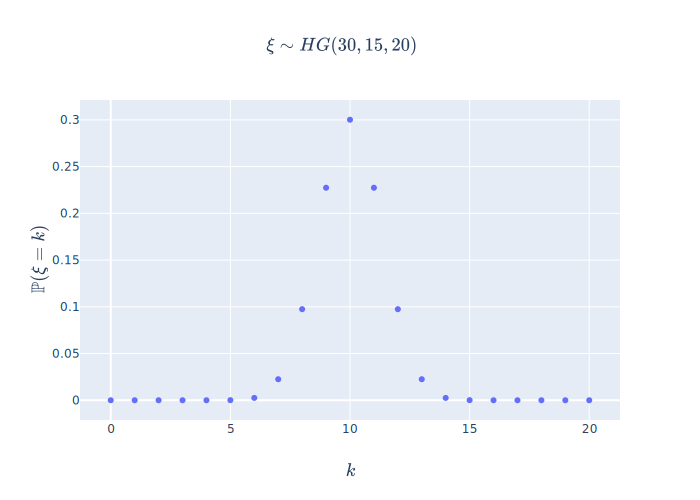
\includegraphics{assets/hg_hist.svg}
\caption{Гистограмма вероятностей гипергеометрического распределения}
\end{figure}

\hypertarget{ux444ux443ux43dux43aux446ux438ux44f-ux440ux430ux441ux43fux440ux435ux434ux435ux43bux435ux43dux438ux44f-ux433ux438ux43fux435ux440ux433ux435ux43eux43cux435ux442ux440ux438ux447ux435ux441ux43aux43eux433ux43e-ux440ux430ux441ux43fux440ux435ux434ux435ux43bux435ux43dux438ux44f}{%
\subsubsection{Функция распределения гипергеометрического
распределения}\label{ux444ux443ux43dux43aux446ux438ux44f-ux440ux430ux441ux43fux440ux435ux434ux435ux43bux435ux43dux438ux44f-ux433ux438ux43fux435ux440ux433ux435ux43eux43cux435ux442ux440ux438ux447ux435ux441ux43aux43eux433ux43e-ux440ux430ux441ux43fux440ux435ux434ux435ux43bux435ux43dux438ux44f}}

По определению, функция распределения
\(F_\xi(k) = \mathbb{P}\left(\, \xi < k \,\right)\). Событие
\(\{\xi < k\} = \bigcup\limits_{i=0}^{k-1}\{\xi=i\}\). События
\(\{\xi=i\}\; \forall i \in \overline{0, k-1}\) являются попарно
несовместными. То есть \(\forall i,j \in \overline{0, k-1}: i \neq j\)
выполняется \(\{\xi=i\}\cap\{\xi=j\}=\emptyset\). Из этого следует, что
\[\mathbb{P}\left(\, \xi < k \,\right) = \sum_{i=0}^{k-1}\mathbb{P}\left(\, \xi = i \,\right)\]
Подставим TODO в это выражение и получим: \[F_\xi(k)
= \sum_{i=0}^{k-1}\mathbb{P}\left(\, \xi = i \,\right)
= \sum_{i=0}^{k-1}\frac{\binom{m}{i}\binom{N-m}{n-i}}{\binom{N}{n}}\]

Построим график этой функции, учитывая, что аргументом \(k\) должно быть
натуральное число, не превосходящее \(n\):

TODO

\hypertarget{ux43dux43eux440ux43cux430ux43bux44cux43dux43eux435-ux440ux430ux441ux43fux440ux435ux434ux435ux43bux435ux43dux438ux435}{%
\subsection{Нормальное
распределение}\label{ux43dux43eux440ux43cux430ux43bux44cux43dux43eux435-ux440ux430ux441ux43fux440ux435ux434ux435ux43bux435ux43dux438ux435}}

Нормальное распределение - непрерывное распределение, описывающее
поведение величины отклонения измеряемого значения \(x\) от истинного
значения \(\mu\) (которое является математическим ожиданием) и в рамках
некоторого разброса \(\sigma\) (среднеквадратичного отклонения). Запишем
это формально: \[\begin{gathered}
    \left\{ \eta \sim N(\mu, \sigma^2) \right\}\\
    \Updownarrow\\
    \left\{\begin{gathered}
        F_\eta(x) = \mathbb{P}\left(\, \eta < x \,\right) = \int_{-\infty}^{x} f_\eta(x)dx,\\
        \text{где} f_\eta(x) = \frac{1}{\sigma\sqrt{2\pi}}e^{-\frac{(x-\mu)^2}{2\sigma^2}}
    \end{gathered}\right\}
\end{gathered}\] \(f_\eta(x)\) называется плотностью вероятности.

\hypertarget{ux43cux430ux442ux435ux43cux430ux442ux438ux447ux435ux441ux43aux43eux435-ux43eux436ux438ux434ux430ux43dux438ux435-ux43dux43eux440ux43cux430ux43bux44cux43dux43eux433ux43e-ux440ux430ux441ux43fux440ux435ux434ux435ux43bux435ux43dux438ux44f}{%
\subsubsection{Математическое ожидание нормального
распределения}\label{ux43cux430ux442ux435ux43cux430ux442ux438ux447ux435ux441ux43aux43eux435-ux43eux436ux438ux434ux430ux43dux438ux435-ux43dux43eux440ux43cux430ux43bux44cux43dux43eux433ux43e-ux440ux430ux441ux43fux440ux435ux434ux435ux43bux435ux43dux438ux44f}}

Найдем математическое ожидание \(\eta \sim N(\mu, \sigma^2)\):
\[\begin{aligned}
    \mathbb{E}\left[\, \eta \,\right] &= \int_{-\infty}^{+\infty} x \cdot f_\eta(x)dx =\\
                  &= \int_{-\infty}^{+\infty} xe^{-\frac{(x-\mu)^2}{2\sigma^2}}dx =\\
                  &= \frac{1}{\sigma\sqrt{2\pi}} \int_{-\infty}^{+\infty} xe^{-\frac{(x-\mu)^2}{2\sigma^2}}dx
\end{aligned}\] Сделаем замену \(t = \frac{x-\mu}{\sqrt{2}\sigma}\):
\[\begin{aligned}
    \mathbb{E}\left[\, \eta \,\right] &= \frac{1}{\sigma\sqrt{2\pi}} \int_{-\infty}^{+\infty}(\sigma\sqrt{2}t + \mu)
                    e^{-t^2} d\left(\frac{x-\mu}{\sqrt{2}\sigma}\right) =\\
                  &= \frac{\sigma\sqrt{2}}{\sqrt{\pi}}\int_{-\infty}^{+\infty}te^{-t^2}dt
                    + \frac{\mu}{\sqrt{\pi}}\int_{-\infty}^{+\infty}e^{-t^2}dt =\\
                  &= \frac{\sigma\sqrt{2}}{\sqrt{\pi}}\left(\int_{-\infty}^{0}te^{-t^2}dt
                    - \int_{-\infty}^{0}te^{-t^2}dt\right) + \frac{\mu}{\sqrt{\pi}}\int_{-\infty}^{+\infty}e^{-t^2}dt =\\
                  &= \frac{\mu}{\sqrt{\pi}}\int_{-\infty}^{+\infty}e^{-t^2}dt
\end{aligned}\] Заметим, что получившееся выражение содержит интеграл,
который может быть сведен к интегралу
\href{https://ru.wikipedia.org/wiki/Гауссов_интеграл}{Эйлера-Пуассона}:
\[\int_{-\infty}^{+\infty}e^{-t^2}dt = 2\int_{0}^{+\infty}e^{-t^2}dt = \sqrt{\pi}\]
Таким образом, \[\boxed{
    \mathbb{E}\left[\, \eta \,\right] = \mu
}\]

\hypertarget{ux434ux438ux441ux43fux435ux440ux441ux438ux44f-ux43dux43eux440ux43cux430ux43bux44cux43dux43eux433ux43e-ux440ux430ux441ux43fux440ux435ux434ux435ux43bux435ux43dux438ux44f}{%
\subsubsection{Дисперсия нормального
распределения}\label{ux434ux438ux441ux43fux435ux440ux441ux438ux44f-ux43dux43eux440ux43cux430ux43bux44cux43dux43eux433ux43e-ux440ux430ux441ux43fux440ux435ux434ux435ux43bux435ux43dux438ux44f}}

Подставим TODO в определение дисперсии TODO: \[\begin{aligned}
    \mathrm{Var}\left[\, \eta \,\right] &= \mathbb{E}\left[\, (\eta - \mu)^2 \,\right] =\\
               &= \int_{-\infty}^{+\infty} (x-\mu)^2 \cdot f_{\eta}(x)dx =\\
               &= \int_{-\infty}^{+\infty}(x-\mu)^2 \frac{1}{\sigma\sqrt{2\pi}}e^{-\frac{(x-\mu)^2}{2\sigma^2}}dx =\\
               &= \frac{1}{\sigma\sqrt{2\pi}}\int_{-\infty}^{+\infty}(x-\mu)^2 e^{-\frac{(x-\mu)^2}{2\sigma^2}}dx
\end{aligned}\] Сделаем ту же замену переменной
\(t = \frac{x-\mu}{\sqrt{2}\sigma}\), тогда \(x = t\sqrt{2}\sigma+\mu\)
и: \[\begin{aligned}
    \mathrm{Var}\left[\, \eta \,\right] &= \frac{1}{\sigma\sqrt{2\pi}}
                \int_{-\infty}^{+\infty}(\sqrt{2}\sigma)^2 t^2 e^{-t^2}d(t\sqrt{2}\sigma+\mu) =\\
               &= \frac{2\sigma^2}{\sqrt{\pi}}\int_{-\infty}^{+\infty}t^2 e^{-t^2}dt
\end{aligned}\] Проинтегрируем по частям: \[\begin{aligned}
    \mathrm{Var}\left[\, \eta \,\right] &= \frac{\sigma^2}{\sqrt{\pi}}\int_{-\infty}^{+\infty}t 2t e^{-t^2} dt =\\
               &= \frac{\sigma^2}{\sqrt{\pi}}\left(\left. -t e^{-t^2} \right|_{-\infty}^{+\infty}
                 + \int_{-\infty}^{+\infty}e^{-t^2}dt\right)
\end{aligned}\] Здесь снова появляется интеграл
\href{https://ru.wikipedia.org/wiki/Гауссов_интеграл}{Эйлера-Пуассона}
и, в итоге, получаем: \[\boxed{
    \mathrm{Var}\left[\, \eta \,\right] = \sigma^2
}\] То есть, \(\sigma\) является среднеквадратичным отклонением.

\begin{lstlisting}[language=Python]
def f() -> int:
    if 1 != 2:
        print("mitinarseny@gmail.com -> abc")
\end{lstlisting}

\end{document}
